\documentclass[10pt,aspectratio=169,serif]{ctexbeamer}

%\usepackage[fontset=none, scheme=plain]{ctex}
\IfFontExistsTF{Songti SC}{%
	\setCJKmainfont{Songti SC}[AutoFakeSlant=0.2]%
	\setCJKsansfont{Songti SC}[AutoFakeSlant=0.2]%
}{%
	\setCJKmainfont{FandolSong-Regular}[Extension=.otf,BoldFont=FandolSong-Bold,AutoFakeSlant=0.2]%
	\setCJKsansfont{FandolSong-Regular}[Extension=.otf,BoldFont=FandolSong-Bold]%
}
\usepackage{amsmath,amssymb,graphicx,tikz,booktabs,multicol,calligra}
\usepackage{pgfplots}
\pgfplotsset{compat=1.18}
\usepackage{tcolorbox}
\tcbuselibrary{skins}
\usepackage{XyygU}
\usepackage{caption}
\captionsetup[figure]{name=图,labelsep=period}

\usetikzlibrary{arrows.meta,positioning,calc}

\setlength{\abovedisplayskip}{0pt plus 2pt minus 2pt}
\setlength{\belowdisplayskip}{0pt plus 2pt minus 2pt}

\title[4.2 指数函数 练习]{4.2 指数函数（课后练习）}
\subtitle{4.2.1 概念 \,$\cdot$\, 4.2.2 图象与性质}
\author{}
\institute{}
\date{2026-10-16}

\begin{document}

\begin{frame}
  \titlepage
\end{frame}

% ============== 4.2.1 练习 ==============
\begin{frame}[t]{4.2.1 练习 第1题：识别指数函数图象}
\textbf{1.} 下列图象中，有可能表示指数函数的是（\quad）。

\begin{center}
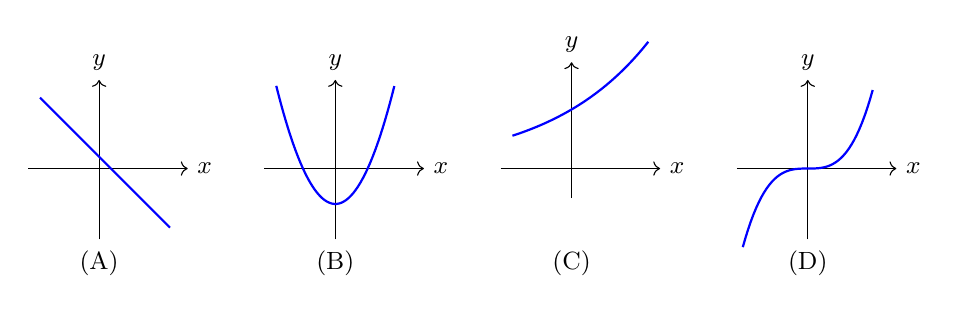
\begin{tikzpicture}[scale=0.75]
% A: 直线下降
\begin{scope}[shift={(0,0)}]
  \draw[->] (-1.2,0)--(1.5,0) node[right]{\small $x$};
  \draw[->] (0,-1.2)--(0,1.5) node[above]{\small $y$};
  \draw[thick,blue] (-1,1.2)--(1.2,-1);
  \node at (0,-1.6){\small (A)};
\end{scope}
% B: 抛物线
\begin{scope}[shift={(4,0)}]
  \draw[->] (-1.2,0)--(1.5,0) node[right]{\small $x$};
  \draw[->] (0,-1.2)--(0,1.5) node[above]{\small $y$};
  \draw[thick,blue,domain=-1:1,samples=50] plot (\x,{2*\x*\x-0.6});
  \node at (0,-1.6){\small (B)};
\end{scope}
% C: 递增过(0,1)
\begin{scope}[shift={(8,0)}]
  \draw[->] (-1.2,0)--(1.5,0) node[right]{\small $x$};
  \draw[->] (0,-0.5)--(0,1.8) node[above]{\small $y$};
  \draw[thick,blue,domain=-1:1.3,samples=50] plot (\x,{pow(1.8,\x)});
  \node at (0,-1.6){\small (C)};
\end{scope}
% D: 过原点
\begin{scope}[shift={(12,0)}]
  \draw[->] (-1.2,0)--(1.5,0) node[right]{\small $x$};
  \draw[->] (0,-1.2)--(0,1.5) node[above]{\small $y$};
  \draw[thick,blue,domain=-1.1:1.1,samples=50] plot (\x,{pow(\x,3)});
  \node at (0,-1.6){\small (D)};
\end{scope}
\end{tikzpicture}
\end{center}
\end{frame}

\begin{frame}[t]{4.2.1 练习 第1题 解答}
\begin{tcolorbox}[colback=orange!10,colframe=orange,title=\textbf{解}]
指数函数 $y=a^{x}\ (a>0,a\ne 1)$ 必满足：
\begin{itemize}
  \item 定义域为 $\mathbf{R}$，图象向左右两方无限延伸；
  \item 图象恒过定点 $(0,1)$，即 $x=0$ 时 $y=1$；
  \item 当 $a>1$ 时单调递增，当 $0<a<1$ 时单调递减；
  \item 函数值恒为正，图象在 $x$ 轴上方。
\end{itemize}

\vspace{0.4em}
(A) 是直线（一次函数）；(B) 是抛物线（二次函数）；
(D) 图象过原点 $(0,0)$，不满足过 $(0,1)$。只有 (C) 是递增且过 $(0,1)$ 的曲线。

\vspace{0.4em}
\textbf{答案：C。}
\end{tcolorbox}
\end{frame}

% ========== 第2题 ==========
\begin{frame}[t]{4.2.1 练习 第2题：求指数函数解析式}
\textbf{2.} 已知函数 $y=f(x),\ x\in\mathbf{R}$，且 $f(0)=3$，
\[
\frac{f(0.5)}{f(0)}=2,\quad \frac{f(1)}{f(0.5)}=2,\quad\cdots,\quad
\frac{f(0.5n)}{f(0.5(n-1))}=2,\quad n\in\mathbf{N}^{*},
\]
求函数 $y=f(x)$ 的一个解析式。
\end{frame}

\begin{frame}[t]{4.2.1 练习 第2题 解答}
\begin{tcolorbox}[colback=orange!10,colframe=orange,title=\textbf{解}]
由题意，自变量每增加 $0.5$，函数值就变为原来的 $2$ 倍，即
\[
f(x+0.5)=2\,f(x).
\]
设 $f(x)=3a^{x}$（由 $f(0)=3$ 得系数为 $3$），则
\[
f(x+0.5)=3a^{x+0.5}=a^{0.5}\cdot 3a^{x}=a^{0.5}f(x)=2f(x),
\]
故 $a^{0.5}=2$，解得 $a=4$。

\vspace{0.6em}
所以
\[
\alert{f(x)=3\cdot 4^{x}=3\cdot 2^{2x}}.
\]

\vspace{0.4em}
\small（验证：$f(0)=3,\ f(0.5)=3\cdot 2=6,\ f(1)=12$，相邻两项之比均为 $2$，符合题意。）
\end{tcolorbox}
\end{frame}

% ========== 第3题 ==========
\begin{frame}[t]{4.2.1 练习 第3题：蓝藻增长}
\textbf{3.} 在某个时期，某湖泊中的蓝藻每天以 $6.25\%$ 的增长率呈指数增长，那么经过 $30$ 天，该湖泊的蓝藻会变为原来的多少倍？（可以使用计算工具）
\end{frame}

\begin{frame}[t]{4.2.1 练习 第3题 解答}
\begin{tcolorbox}[colback=orange!10,colframe=orange,title=\textbf{解}]
设原有蓝藻量为 $N_{0}$，经过 $x$ 天后蓝藻量为
\[
N(x)=N_{0}(1+6.25\%)^{x}=N_{0}\cdot 1.0625^{x}.
\]
当 $x=30$ 时，
\[
N(30)=N_{0}\cdot 1.0625^{30}.
\]
用计算工具：
\[
1.0625^{30}\approx 6.13.
\]
所以经过 $30$ 天，该湖泊的蓝藻约变为原来的 $\alert{6.13}$ 倍。
\end{tcolorbox}
\end{frame}

% ============== 4.2.2 练习 ==============
\begin{frame}[t]{4.2.2 练习 第1题：$y=3^{x}$ 与 $y=\left(\frac{1}{3}\right)^{x}$}
\textbf{1.} 在同一直角坐标系中画出函数 $y=3^{x}$ 和 $y=\left(\dfrac{1}{3}\right)^{x}$ 的图象，并说明它们的关系。
\end{frame}

\begin{frame}[t]{4.2.2 练习 第1题 图象}
\begin{center}
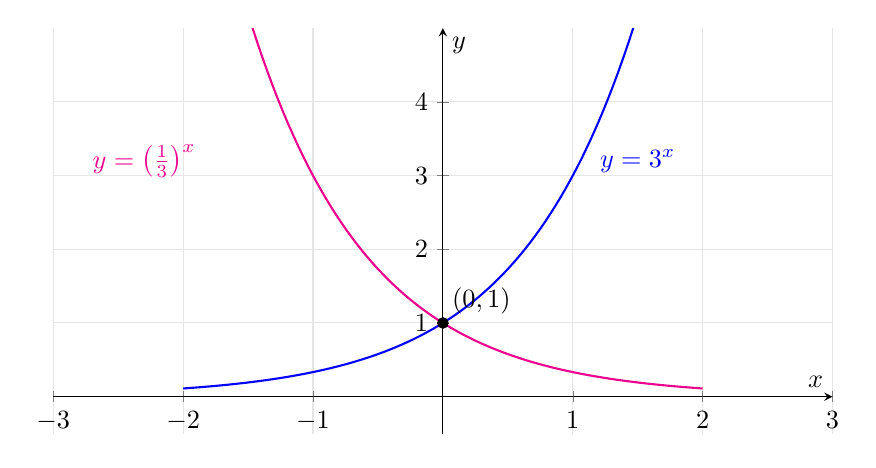
\begin{tikzpicture}[scale=0.95]
\begin{axis}[
    width=12cm, height=7cm,
    axis lines=middle,
    xlabel=$x$, ylabel=$y$,
    xmin=-3, xmax=3, ymin=-0.5, ymax=5,
    xtick={-3,-2,-1,0,1,2,3},
    ytick={1,2,3,4},
    grid=major, grid style={gray!20},
]
\addplot[thick,blue,domain=-2:2,samples=100] {3^x};
\addplot[thick,magenta,domain=-2:2,samples=100] {0.333333^x};
\addplot[only marks,mark=*,mark size=2pt,black] coordinates {(0,1)};
\node[blue] at (axis cs:1.5,3.2) {$y=3^{x}$};
\node[magenta] at (axis cs:-2.3,3.2) {$y=\left(\frac{1}{3}\right)^{x}$};
\node[above right] at (axis cs:0,1) {$(0,1)$};
\end{axis}
\end{tikzpicture}
\end{center}
\end{frame}

\begin{frame}[t]{4.2.2 练习 第1题 解答}
\begin{tcolorbox}[colback=orange!10,colframe=orange,title=\textbf{解}]
因为
\[
\left(\frac{1}{3}\right)^{x}=3^{-x},
\]
所以点 $(x,y)$ 在 $y=3^{x}$ 图象上 $\Longleftrightarrow$ 点 $(-x,y)$ 在 $y=\left(\frac{1}{3}\right)^{x}$ 图象上。

\vspace{0.4em}
因此两个函数的图象\alert{关于 $y$ 轴对称}，且都过定点 $(0,1)$：
\begin{itemize}
  \item $y=3^{x}$ 底数 $3>1$，是 $\mathbf{R}$ 上的增函数；
  \item $y=\left(\frac{1}{3}\right)^{x}$ 底数 $0<\frac{1}{3}<1$，是 $\mathbf{R}$ 上的减函数。
\end{itemize}
\end{tcolorbox}
\end{frame}

% ========== 第2题 ==========
\begin{frame}[t]{4.2.2 练习 第2题：比较大小}
\textbf{2.} 比较下列各题中两个值的大小：
\[
(1)\ 6^{\sqrt{2}},\ 7^{\sqrt{2}};\qquad
(2)\ 0.3^{-3.5},\ 0.3^{-2.3};\qquad
(3)\ 1.2^{0.5},\ 0.5^{1.2}.
\]
\end{frame}

\begin{frame}[t]{4.2.2 练习 第2题 解答}
\begin{tcolorbox}[colback=orange!10,colframe=orange,title=\textbf{解}]
\textbf{(1)} 把它们看作幂函数 $y=x^{\sqrt{2}}$（$\sqrt{2}>0$，在 $x>0$ 时单调递增）的两个函数值。
因为 $6<7$，所以 $\alert{6^{\sqrt2}<7^{\sqrt2}}$。

\vspace{0.5em}
\textbf{(2)} 看作指数函数 $y=0.3^{x}$（底数 $0<0.3<1$，单调递减）。
因为 $-3.5<-2.3$，递减函数自变量小则函数值大，所以 $\alert{0.3^{-3.5}>0.3^{-2.3}}$。

\vspace{0.5em}
\textbf{(3)} 借助中间量 $1$：
\[
1.2^{0.5}>1.2^{0}=1,\qquad 0.5^{1.2}<0.5^{0}=1,
\]
所以 $\alert{1.2^{0.5}>0.5^{1.2}}$。
\end{tcolorbox}
\end{frame}

% ========== 第3题 ==========
\begin{frame}[t]{4.2.2 练习 第3题：癌细胞增长示意图}
\textbf{3.} 体内癌细胞初期增加得很缓慢，但到了晚期就急剧增加，画一幅能反映体内癌细胞数量随时间变化的示意图。
\end{frame}

\begin{frame}[t]{4.2.2 练习 第3题 解答}
\begin{columns}
\column{0.48\textwidth}
\begin{tcolorbox}[colback=orange!10,colframe=orange,title=\textbf{分析}]
癌细胞数量初期缓慢、晚期急剧增加，正是指数函数
\[
y=a^{x}\quad (a>1)
\]
的典型特征：当 $x$ 较小时曲线平缓，当 $x$ 增大后曲线迅速上升。

\vspace{0.5em}
示意图可设：
\[
N(t)=N_{0}\,a^{t}\quad (a>1),
\]
横轴为时间 $t$，纵轴为癌细胞数量 $N$。
\end{tcolorbox}

\column{0.52\textwidth}
\begin{tikzpicture}[scale=0.85]
\begin{axis}[
    width=7cm, height=6cm,
    axis lines=middle,
    xlabel=$t$, ylabel=$N$,
    xmin=0, xmax=6, ymin=0, ymax=5,
    xtick={}, ytick={},
]
\addplot[thick,blue,domain=0:5,samples=100] {0.5*exp(0.7*x)};
\node[blue] at (axis cs:4.2,3.8) {$N(t)=N_{0}a^{t}$};
\node[below left] at (axis cs:0,0) {$O$};
\end{axis}
\end{tikzpicture}
\end{columns}
\end{frame}

\begin{frame}[c]
  \begin{center}
    {\Huge\calligra Thanks!}
  \end{center}
\end{frame}

\end{document}
